\olge{I think this section is way too long - it's still background information, not the actual proposal. In my opinion we should (1) concisely discuss the AS-relevant properties of DR (max one page), then (2) make the case for the rest of the paper in {\ref{subsec:unused}} - i.e. we're underutilizing the capabilities of these new resources because the service definitions were made for the previous generation of power systems. Permission to slash? :-)}
\bondy{Technical Properties of Unconventional Resources for Ancillary Service Delivery}

\subsection{The properties of DR}
Here we argue that DR (and other new technologies) have additional degrees of freedom with respect to shaping the response to an ancillary services request, compared to traditional generators.

\iffalse %Section commented out for the moment - I think it doesn't fit the current/new purpose of this chapter but at least some of it would probably fit well closer to the end of the paper. We'll propose a service definition; part of that proposal should be a discussion on how it could be adopted. Listing existing barriers would be a natural introduction to this discussion IMHO -olge 31/7/2015

%%%%%%%%%%%%%%%%%%%%%%%%%%
\subsubsection{Barriers for demand response in the ancillary service markets}\label{sec:drinasm}
%%%%%%%%%%%%%%%%%%%%%%%%%%
\textcolor{red}{Jason: I need your help here!, given the turn of the paper, I'm not sure how relevant this subsection is. We might need to delete it.}

Currently, DR is not widespread in the ancillary service markets. In Europe, DR has had some difficulty entering the energy markets. In a report from 2014 \cite{sedc2014mapping}, it is shown that only Belgium, Great Britain, Finland, France, Ireland and Switzerland have regulatory framework that permits DR to be viable. This is in part due to the requirements presented in section~\ref{sec:procurement}.

In most ancillary service markets that accept demand response (DR) participation, the requirements for participation, as well as the verification and settlement, are equal to those of traditional generation units, e.g. \cite{energinet2012ancillary} \textcolor{red}{(we need more examples, or a source that is more explicit about it)}. That means that an aggregator participating in an ancillary service market must behave as if it is a single large unit, and not a composition of many smaller units \textcolor{red}{(maybe this sentence should come in the introduction)}. 
%This is exemplified in the Nordic countries:
%\begin{quote}
%	[\ldots]the TSOs agree that aggregation of smaller consumption units is necessary as, for the time being, it is not expedient to include very small bids \cite{energinet2013amendment}.
%\end{quote}

PJM is an exception to a few of the previous statements, in that it has implemented DR remuneration through mileage payment options \cite{pjm2015energy}.

There are markets where DR is not allowed to participate in the ancillary service markets. This restriction is either due to technical issues \textcolor{red}{(examples)} or due to regulatory issues \textcolor{red}{(examples)}. An overview of the state of Demand Response in Europe is presented in \cite{sedc2014mapping}, and although the analysis is not focused on Demand Response participation for AS, it gives an idea of the challenges Europe faces to introduce DR in the energy markets.
\fi

\subsubsection{Demand-side resources}
\olge{I think this should be shortened radically. The point is not to give a comprehensive overview of DR but to show what DR can do. IMHO we could get better mileage if we just gave best-in-class examples for the different properties, e.g. a type of resource that can respond very fast, another one with minimal cycling constraints etc. etc. It's clear (or we could make it clear) that a real-world portfolio will contain a mix of such resources, but also that portfolios could be optimized towards particular properties.}
The demand-side resources (DSRs) that can provide DR vary greatly in composition, and each have their own properties. Most of the research on DR to provide transmission level services have focused on specific services using a particular set of loads connected to the grid. This is partly due to varying characteristics of DSRs and partly because of the suitable control architecture for the proposed services. In this study, our goal is to identify DR characteristics, similar to \cite{oldewurtel2013framework}, and capture different the properties of DSRs from a transmission-level benefits perspective. The motivation behind is to support an objective and comprehensive comparison between traditional AS providers and DSRs. 

\paragraph{Thermal loads}
A common set of resources studied in connection to DR are thermostatically controlled loads~\cite{Molina_Garcia_2011,Kara_2012}, such as electric space heating \cite{mathieu2012using,thavlov2014utilization}, residential and industrial refrigeration \cite{lakshmanan2014energy} and space heating using heat pumps \cite{halvgaard2012economic}. This is due to the inherent heat inertia present in the systems where these resources perform. The heat inertia acts as energy storage, permitting the curtailment or deferral of power consumption. This also applies to industrial applications such as large refrigeration systems \cite{rahnama2013integration}, the heating of bitumen tanks \cite{cheng2014availability} and indoor climate control using HVAC \cite{blum2013ancillary}. These units typically have a fast response time, and depending on the state of the unit will have short to medium duration capabilities. In all cases it is an energy service which is deferrable, except in the HVAC case, where one could make an argument that in some areas, with wide temperature differences between day and night, the power not used during the day will not be used later, since the ambient temperature will have decreased enough to be comfortable to the unit owner. \textcolor{red}{(This is a corner case, is it worth mentioning?)} These units typically have a cycling constraint in order to protect the compressors and pumps, although this is not the case of electric space heating \textcolor{red}{as far as I know}.

\paragraph{Electric vehicles and batteries}
Another resource that can provide DR are batteries. Electric vehicles (EVs) can be considered as batteries with mobility and extra time varying constraints. By changing their charge patterns, within the comfort bounds of the owner, the EVs can provide frequency control services to the TSO \cite{zarogiannis2014dynamic} \textcolor{red}{(Maybe Emre wants to plug some of his research here)}. The response time is fast, and depending on the size and state of the unit/portfolio, the duration capabilities are medium to long. The EV consumes energy and its consumption is deferrable. The charging of EVs has no cycling constraint.
\paragraph{Lighting}
In \cite{rubinstein2011demand} a study is presented showing the expected potential of using the dimming of lighting in office buildings for DR. Also, a pilot project in Denmark used the lighting of an industrial green house for DR [cite], showing the potential of using DR for congestion management in the distribution system. These units provide fast response, and depending on which kind of load decrease they perform (light dimming or switching off), they can either sustain it for short, medium or large periods. Generally, lighting is a power service which curtailable, but in the case of the green houses it is actually an energy service that is deferrable.
\paragraph{Pump systems}
A new resource for flexibility has been found in systems using water pumps. An example is waste water treatment plants [cite: Halvgaard], where water is transported by pumps to stations for cleaning. In this case the power consumption flexibility stems from the fact that water can be temporarily stored in the pipe system and transported to the cleaning center at a later moment, plus 50\% of the energy consumption of a waste water treatment plant is spent on the aeration process, which can be deferred. Another example is the water pumping in agricultural systems, where there is flexibility with regards to the time of irrigation. The response of the pumps is fast, and depending on the system state and weather conditions can be sustained from medium to long time. The system requires a certain amount of energy to move the water around, and is therefore deferrable. Due to the pumps there may be constraints on the cycling.

\subsubsection{Demand Response Properties}
\olge{We're introducting terminology here that we might need in the proposed service definition. I'm thinking that we might want to limit ourselves to those terms/properties that we need later?}
FERC defines Demand Response (DR) as:
\begin{quote}
	Changes in electric usage by demand-side resources from their normal consumption patterns in response to changes in the price of electricity over time, or to incentive payments designed to induce lower electricity use at times of high wholesale market prices or when system reliability is jeopardized\cite{fercdrdef}.
\end{quote}

In this paper we will be focusing on the last part, i.e., the use of DR when the system reliability is jeopardized. Using DR for helping when system reliability is jeopardized means providing ancillary services with DR. We will assume that AS stemming from DR will be sold to system operators by an aggregator. The properties of aggregating consumption loads will be described in the following subsections.

The identified DSR parameters are given as follows:
\olge{I know I probably spend way too much time looking at microcontroller timing diagrams, but would it help trying to put all the parameters into a single timeline drawing like the sketch in figure {\ref{fig:resourcecharacteristics}} ?}
\begin{figure}[htb!]
\centering
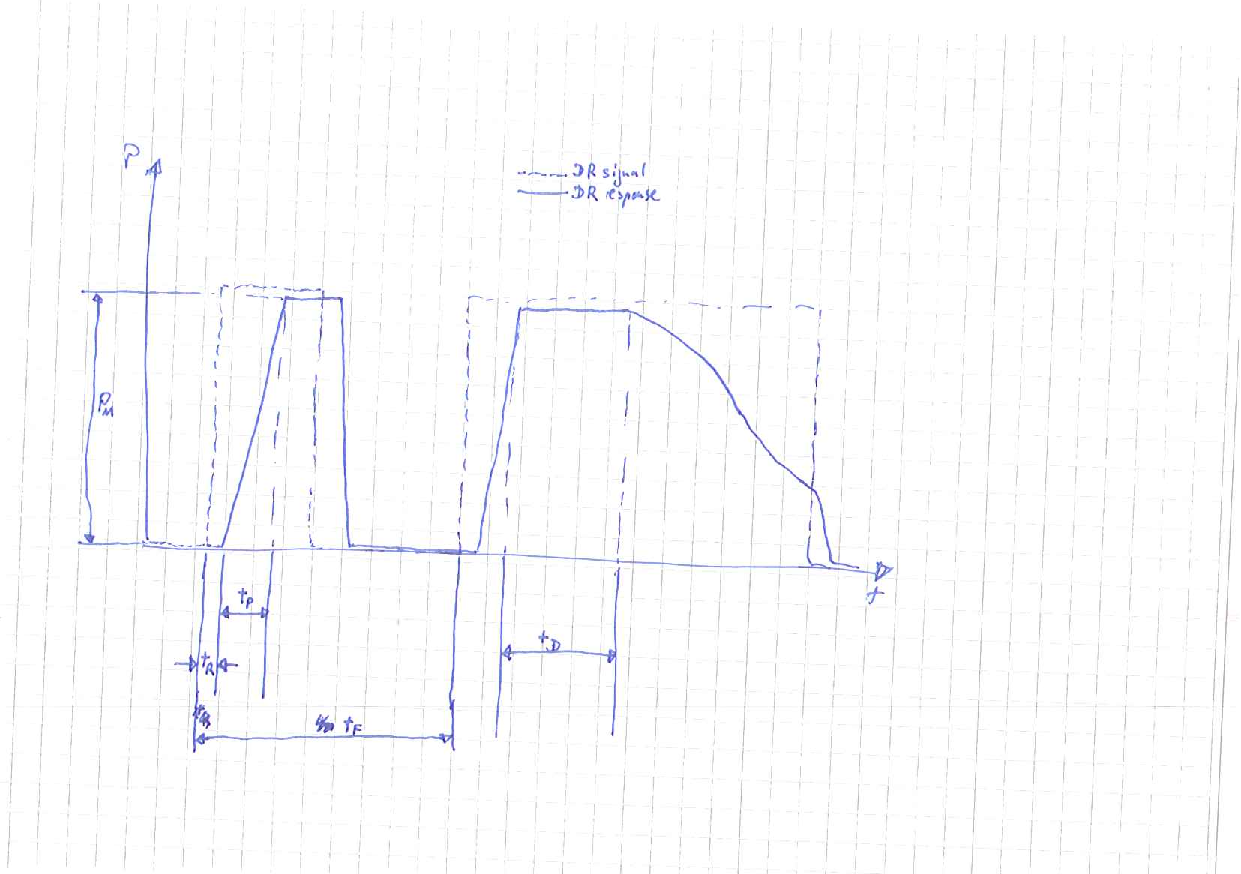
\includegraphics[width=1\columnwidth]{20150731150249153.pdf}
\caption{Characteristics of demand side resources [sketch].}
\label{fig:resourcecharacteristics}
\end{figure}

\begin{description}
	\item[Response time] This is the time it takes for a unit to receive a DR signal and react upon it. \textcolor{red}{I'm not sure on this one, since pretty much all of them have fast response time, depending on the control architecture and the communication system, which are not inherent to the DER}
	\item[Response duration] How long is a pool of these units able to sustain service provision: short, medium or long. \textcolor{red}{Again, this is a tough one, since this will depend on the state of the portfolio/unit}
	\item[Response magnitude] This the \emph{amount} of load used by the DR resources that can be increased or decreased. The increase capability is defined as the \emph{take} magnitude and the decrease capability is defined as the \emph{shed} magnitude.
	\item[Response frequency] The frequency with which the DR resources can be called for service provision. 
	\item[Ramp Rate] The duration necessary for the DR resources to reach the desired response magnitude.
	\item[Response Energy Ratio] The response energy ratio is dependent on the end-use requirements, the time of activation, the amount of energy that is shed or taken during a DR event, and the necessary energy for the load to recover.
Specifically, we define it as the ratio of the energy needed for recovery by the end-use and the energy shed or take during the provisioned DR service.  
	Units providing DR will have as primary objective to satisfy the need of a costumer behavior. This need can be of power, e.g. lighting, and is therefore a curtailable (\textcolor{red}{clippable?}) consumption, or can be an energy need, e.g. space heating, which is usually a deferrable load. Deferrable loads will usually have a kickback effect \cite{han2014load}.
	\item[Cycling constraints] The units' capability to quickly switch between states. Some units may need to rest or settle between changes of state. \olge{I wonder if we aren't mixing different types of characteristics here: Those that are actually reflected in service definitions, like ramp rates and response times, and those that are pure resource constraints like cycling which would be the problem of an aggregator trying to build a portfolio but not visible to e.g. a TSO requesting a service from such a portfolio. Should we separate those?} 
\end{description}

\paragraph{Statistical properties} \label{subsec:statprop}
In \cite{kirby2007load} it is hypothesised \textcolor{red}{(I don't want to use the words proven or shown, since it's not quite what he does)} that the aggregated response of a large number of small loads is more reliable than the response of a few large generating units when responding to a contingency event.

\textcolor{red}{JASON: Talk about measuring 20\% of a portfolio gives enough real time information about the portfolio. What more can we talk about here?}

\iffalse %I commented this out since I don't think it supports the point we're trying to make, which is that aggregates can be more reliable/flexible than single DR units. How the aggregator works isn't really relevant in this context. -olge 31/7/2015
  \paragraph{Architectural properties}
The architecture of the aggregation controller can take several form \cite{kosek2013overview}: 
  \begin{description}
  \item[Direct control] requires two way communication for feedback into the control loop, and gives the aggregator operator better control on the response of the portfolio.
  \item[Indirect control] is a form of open loop control typically based upon price signals. This form of control is less expensive in terms of communication infrastructure, but it is more difficult to predict the response of the portfolio.
  \item[Transactional control] is a control strategy based upon negotiation between the units being aggregated in order to achieve the goal established by the aggregator. The portfolio will find its optimal behavior according to the market designed by the aggragotor.
  \item[Autonomous control] is a decentralized form of control, where each unit reacts to local measurements, and therefore provide a fast response to changes in their environment.
  \end{description}
\fi

\paragraph{Portfolio composition}
Most literature has focused on control of portfolios with a homogeneous population \textcolor{red}{(EMRE: want to cite some of your thermostatic load stuff?)}, or clustered populations [cite e.g. Samira Rahnama or Marco Zugno] with similar properties. The advantage of this is that it simplifies the design of the controller, but it adds the disadvantage of the loads being unavailable at the same time, or a large kick-back effect since they have a similar behavior.

The advantages of heterogeneous portfolios have not been thoroughly analysed. In theory, a portfolio where the units have a wide variety of properties, e.g. fast response of EVs, with a sustained response given by pump systems, will be able to provide better services to the system operators.

\paragraph{Availability \textcolor{red}{(change name?)}}
While the availability for service provision of traditional generation units usually depends only on the normal operation of the generator, and the amount of reserve set aside from the whole sale production, the availability of aggregated units usually has further constraints. This is because the primary function of the DSRs is to satisfy the need of its owner, and within this constraint, provide services to the system operators.

The availability of an aggregator, or the flexibility of the portfolio, depends on factors such as the weather, how much flexibility has already been consumed, the composition of the portfolio, \textcolor{red}{(What else?)}. Conversely, the service delivery by an aggregator is less sensitive to faults in the individual units (see Section \ref{subsec:statprop}).

\paragraph{Performance}
Several studies have been made analysing the performance of service delivery by aggregators, e.g. [cite]. 

The estimated effectiveness of DR is dependant on the baseline model (error). That is, if the behaviour of the DR providing unit is measured against an unrealistic benchmark, it might be confused with the unit not being good at responding to DR signals \cite{mathieu2011variability}.

%\begin{itemize}
%	\item What are the response characteristics of DR?
%		\begin{itemize}
%			\item distributed nature
%			\item aggregated response of many small, several mid-size units and/or a few large units
%			\item reliability and availability
%			\item sources of uncertainty and how to deal with it (adaptation to increasing uncertainty in production may also lead to adaptation to uncertainty in AS)
%		\end{itemize}
%\end{itemize}

\subsection{Unused potential}
\label{subsec:unused}

Here we'll make our central point:
\begin{itemize}
\item DR and other new DER have additional degrees of freedom in terms of response shaping compared to traditional providers of ancillary services
\item The current definition of ancillary services is static/uniform and consequently oriented towards the lowest common denominator (=the resources with the lowest capabilities)
\item In order to continue to accommodate the slowest-ramping thermal power plants while at the same time using the potential of modern DER, ancillary services should either be split up in different service classes, or the service definition should be parametrized
\item A single, parameterizable service definition would be preferable to a set of differentiated services \olge{do we agree on that? What's the line of argumentation?}
\end{itemize}